\section{Method}
\label{sec:method}

%
\begin{figure}
	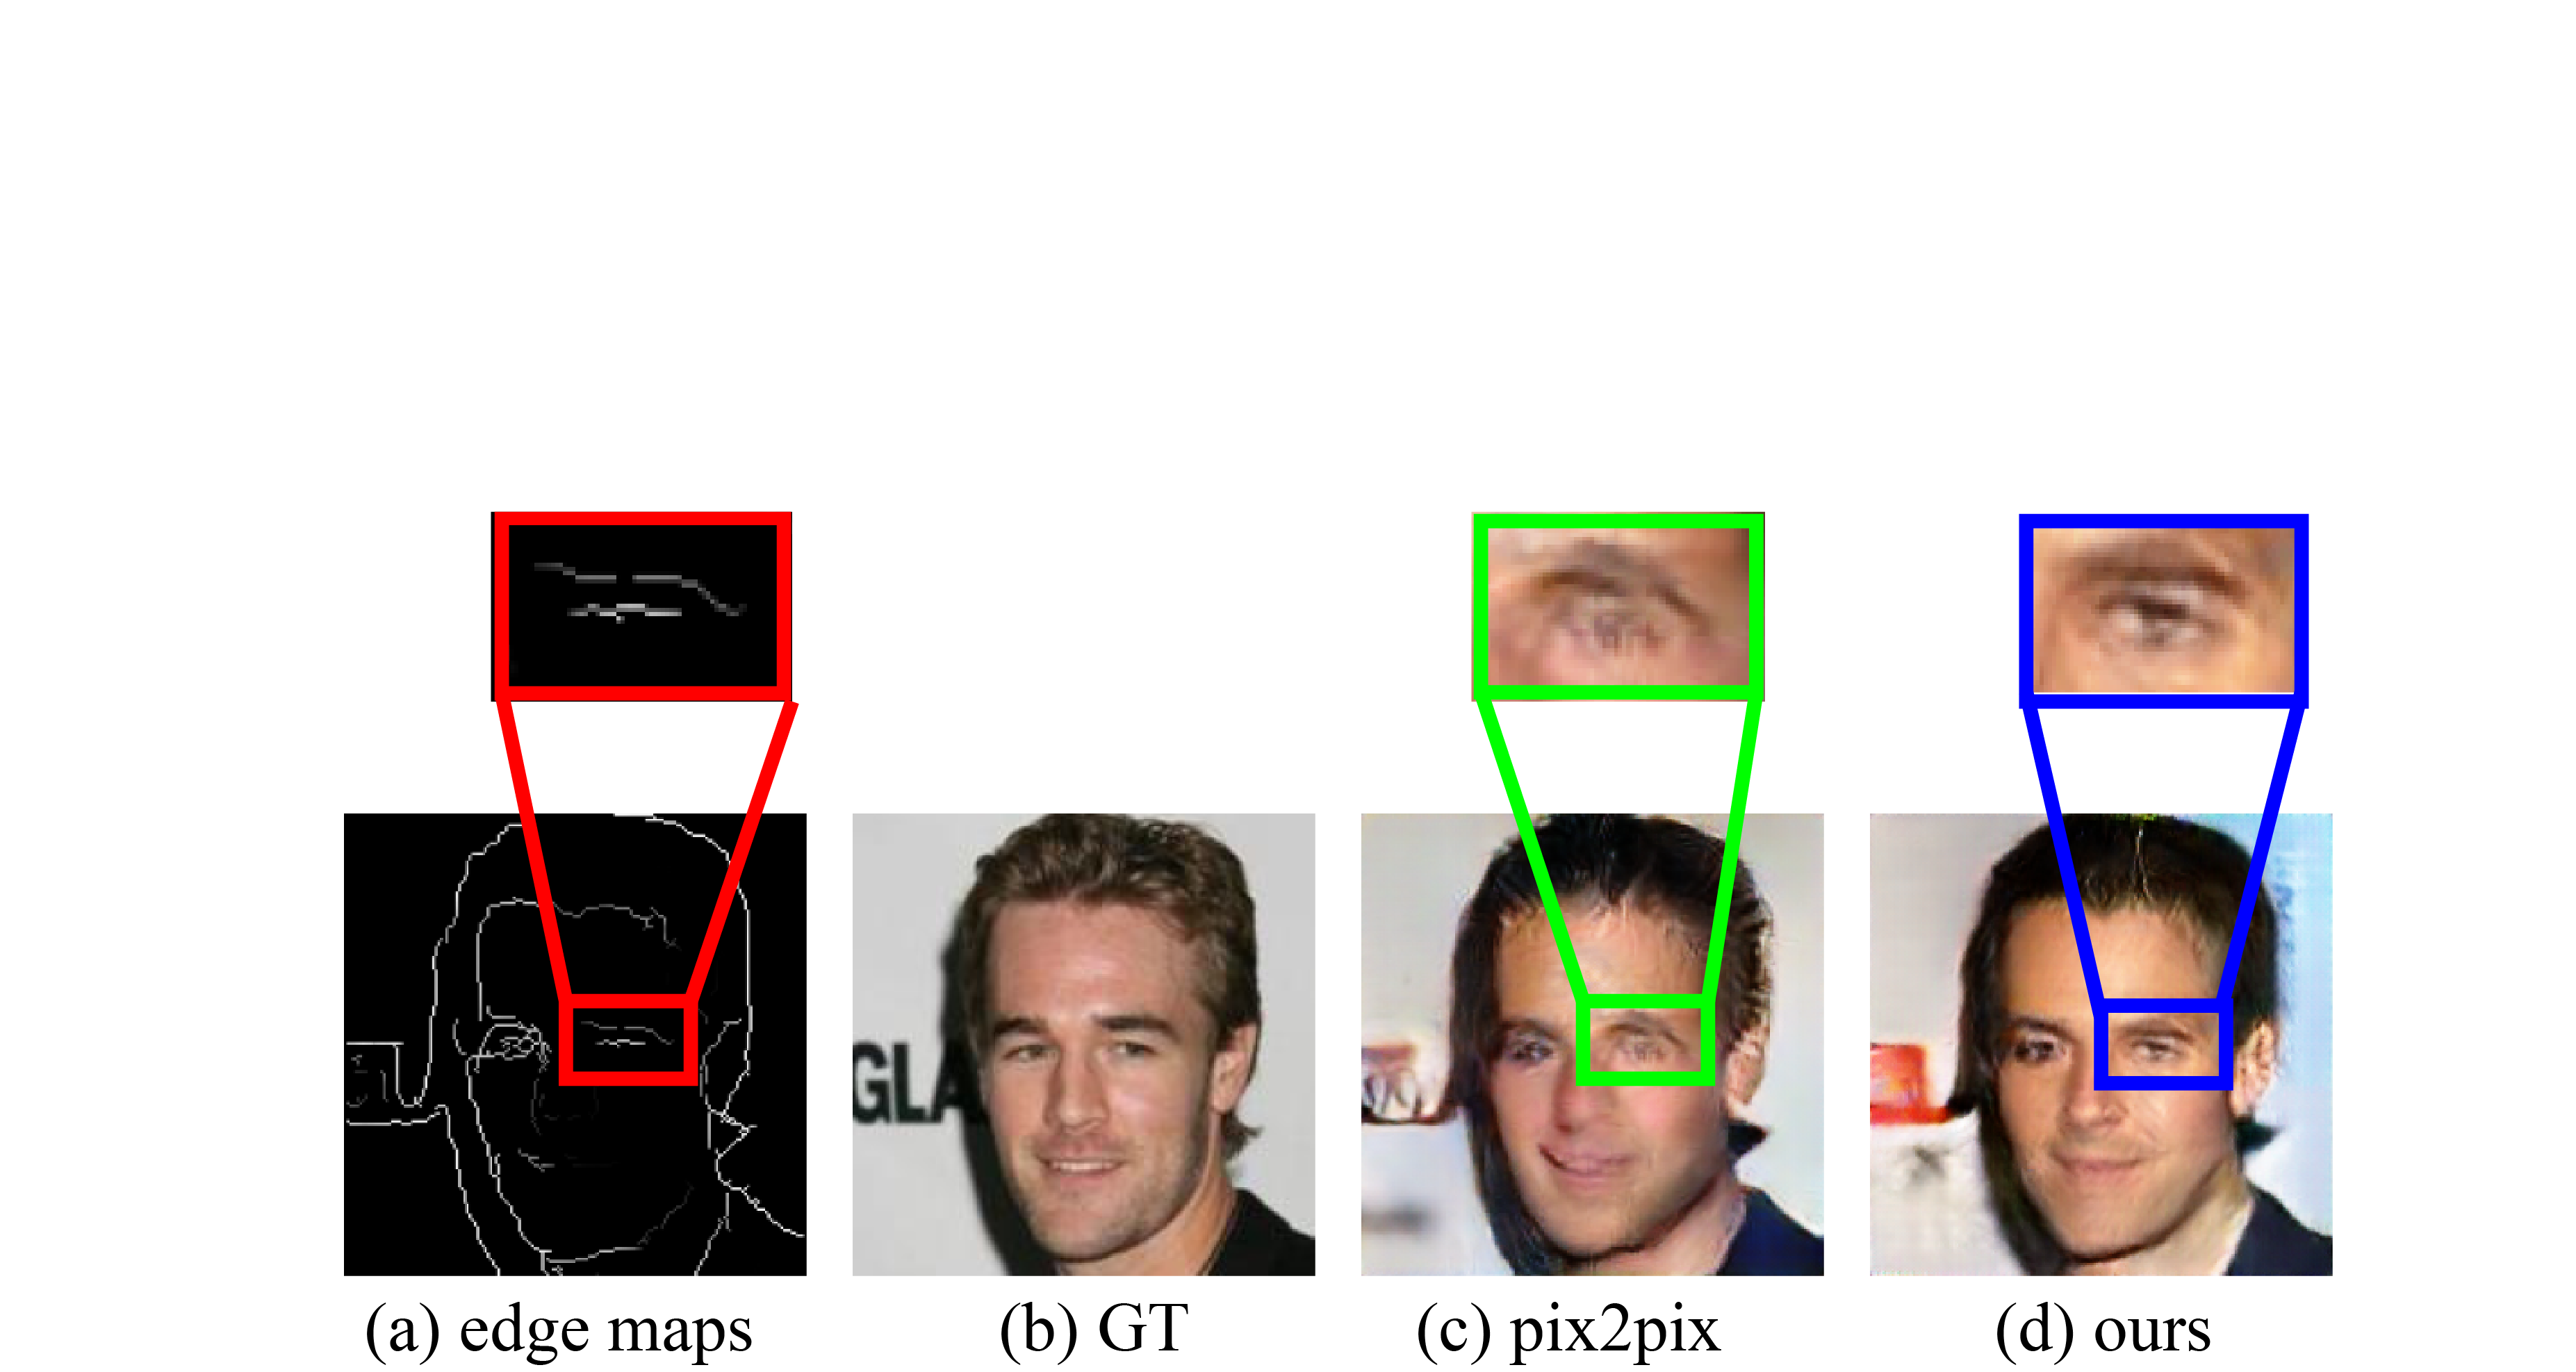
\includegraphics[width=0.8\textwidth]{figures/example}
	\caption{An example of translating face images (b) from the corresponding edge maps (a). In this example, the edge map does not contain the complete edges of the left eye (on the right hand side of the reader). It is obvious that there should be a left eye in the red square according to the global structural information. The pix2pix model (c) fails to render a recognizable eye in the corresponding location (green square) while the proposed method (d) is able to generate the entire structure even when the conditional edge map lacks several parts of the global structure.}
	\label{fig:example}
\end{figure}
%
% too many "long-range dependencies"
The proposed Conditional Self-attention Generative Adversarial Networks (CSAGANs), which translate images from one domain to another and are able to capture long-range dependencies and reserve the global structures across image. We first review the pix2pix model as our baseline (Sec.\ref{subsec:pix2pix}). And then we introduce the Conditional Self-attention Module (SCAM) (Sec. \ref{subsec:CSAM}). Finally, we describe the idea of multiple level patch discriminator (Sec.\ref{subsec:disciminator} and the architecture we proposed (Sec. \ref{subsec:architecture}).
\subsection{The Pix2pix Model}
\label{subsec:pix2pix}
Since our model is based on the pix2pix model \cite{pix2pix}, we review this model in this sub-section. The pix2pix model is an image-to-image translation framework based on conditional GANs, which trains a generator network $G$ and a discriminator network $D$ alternatively. The generator $G$ takes a conditional image as input and outputs the corresponding target image, while the discriminator $D$ distinguishes real images from the synthesized ones. To train these two networks in a supervise manner, a set of corresponding image pairs $\{(\bm{x}_i, \bm{y}_i)\}$ is required as training set, where $\bm{x}_i$ is a conditional image and $\bm{y}_i$ is the corresponding target image. These two networks play a minmax game to guide the generator to model the conditional distribution of real images given the conditional images. The objective is given by:
\begin{equation}
\label{eqn:minmax_game}
\min_G \max_D \mathcal{L}_{adv}(G,D)+\lambda \mathcal{L}_{L1}(G),
\end{equation}
where $G$ aims to minimize this objective while $D$ tries to maximize it inversely.
The adversarial loss function is generally given by 
\begin{equation}
\label{eqn:loss_adv}
\mathcal{L}_{adv}(G,D)=E_{(\bm{x},\bm{y})\sim p_{data}(\bm{x},\bm{y})}[\log D(\bm{x},\bm{y})]+E_{\bm{x}\sim p_{data}(\bm{x})}[\log(1-D(\bm{x},G(\bm{x})))],
\end{equation}
and the $L_1$ loss is given by
\begin{equation}
\label{eqn:loss_l1}
\mathcal{L}_{L1}(G)=\mathbb{E}_{(\bm{x},\bm{y})\sim p_{data}(\bm{x},\bm{y})}[\|\bm{y}-G(\bm{x})\|_1]
\end{equation}
The generator of the pix2pix model is a fully-convolution-based U-Net \cite{Unet}. The input of the generator is only applied to the first layer. The discriminator of the pix2pix model is a patch-wise discriminator, which examines only a patch of its input image and uses the average of outputs from all patches of the input image as the ultimate output. The size of each patch is set to $70\times 70$. The conditional image is concatenated channel-wisely to the synthesized image or real image as the input of the discriminator. 

However, in the task of translating a face image from the corresponding edge map, the pix2pix model has troubles to generate realistic face images in some cases with structural constrains. Since faces have well-defined structural parts, e.g. noses, mouths, eyes and etc., the synthesized face images should contain the whole set of these structural part to be realistic, even when the conditional edge maps lack of edges on the supposed locations of these parts. The pix2pix fails to generate realistic structural part in this circumstance.
% take the first low of the result figure as example
An example is displayed in Figure \ref{fig:example}. In this example, an edge map of a face, shown on the left of the figure, only captures a part of edges of the left eye (in the green square) rather than the whole set of edges of the entire left eye. The face image generated by the pix2pix model on the condition of this edge map is shown on the right in the figure. According to the global structural information, there should be a left eye in the red square obviously. However, we can observe that the pix2pix model fails to render a recognizable left eye in the synthesized face image. 

This phenomenon might be caused by two reasons. 
1) The pix2pix model is a convolution-based model which relies on convolutional operations to model the dependencies across different regions of images and feature maps. Convolutional operations have local receptive fields depending on the kernel sizes and are not able to balance between ability to model long-range dependencies and efficiency of computation and statistics in some cases \cite{SAGANs}.
2) The discriminator used by the pix2pix model is patch-wised, based on the assumption that pixels separated by a distance more than a patch diameter are independent to each other. This assumption is true in some cases like texture generation and style transfer, and has been applied in previous work \cite{texture_markovian, styel_transfer}. However, this assumption fails in the case with global structural constrains. Therefore the patch-wise discriminator fails to grasp the global structure information and is not able to guide the generator to be aware of the structure of the faces.

To address the problem caused by the first reason, we introduce self-attention to the generator of image-to-image models to address the problem.
Self-attention \cite{Non-local, Attention, MachineReading, SAGANs}, which computes the response at a position as a weighted sum of the features at all positions, is able to capture the long-range dependencies across different regions of images and feature maps. In order to adapting the conditional setting of image-to-image translation and encouraging the model to leverage the information of the conditional image directly, we propose a conditional self-attention module (CSAM), which enables the higher layers to sense the conditional image, as a general module of networks.
%
For the second reason, we consider to establish a multi-level discriminator to capture the information of its input image both patch-wisely and globally. We note that similar ideas of multiple discriminators have been raised by \cite{LaplaceGANs, SGANs, StackGANs, CRN} with different architectures. We describe CSAM and the multi-level discriminator in next sections.
%
%
\begin{figure}
	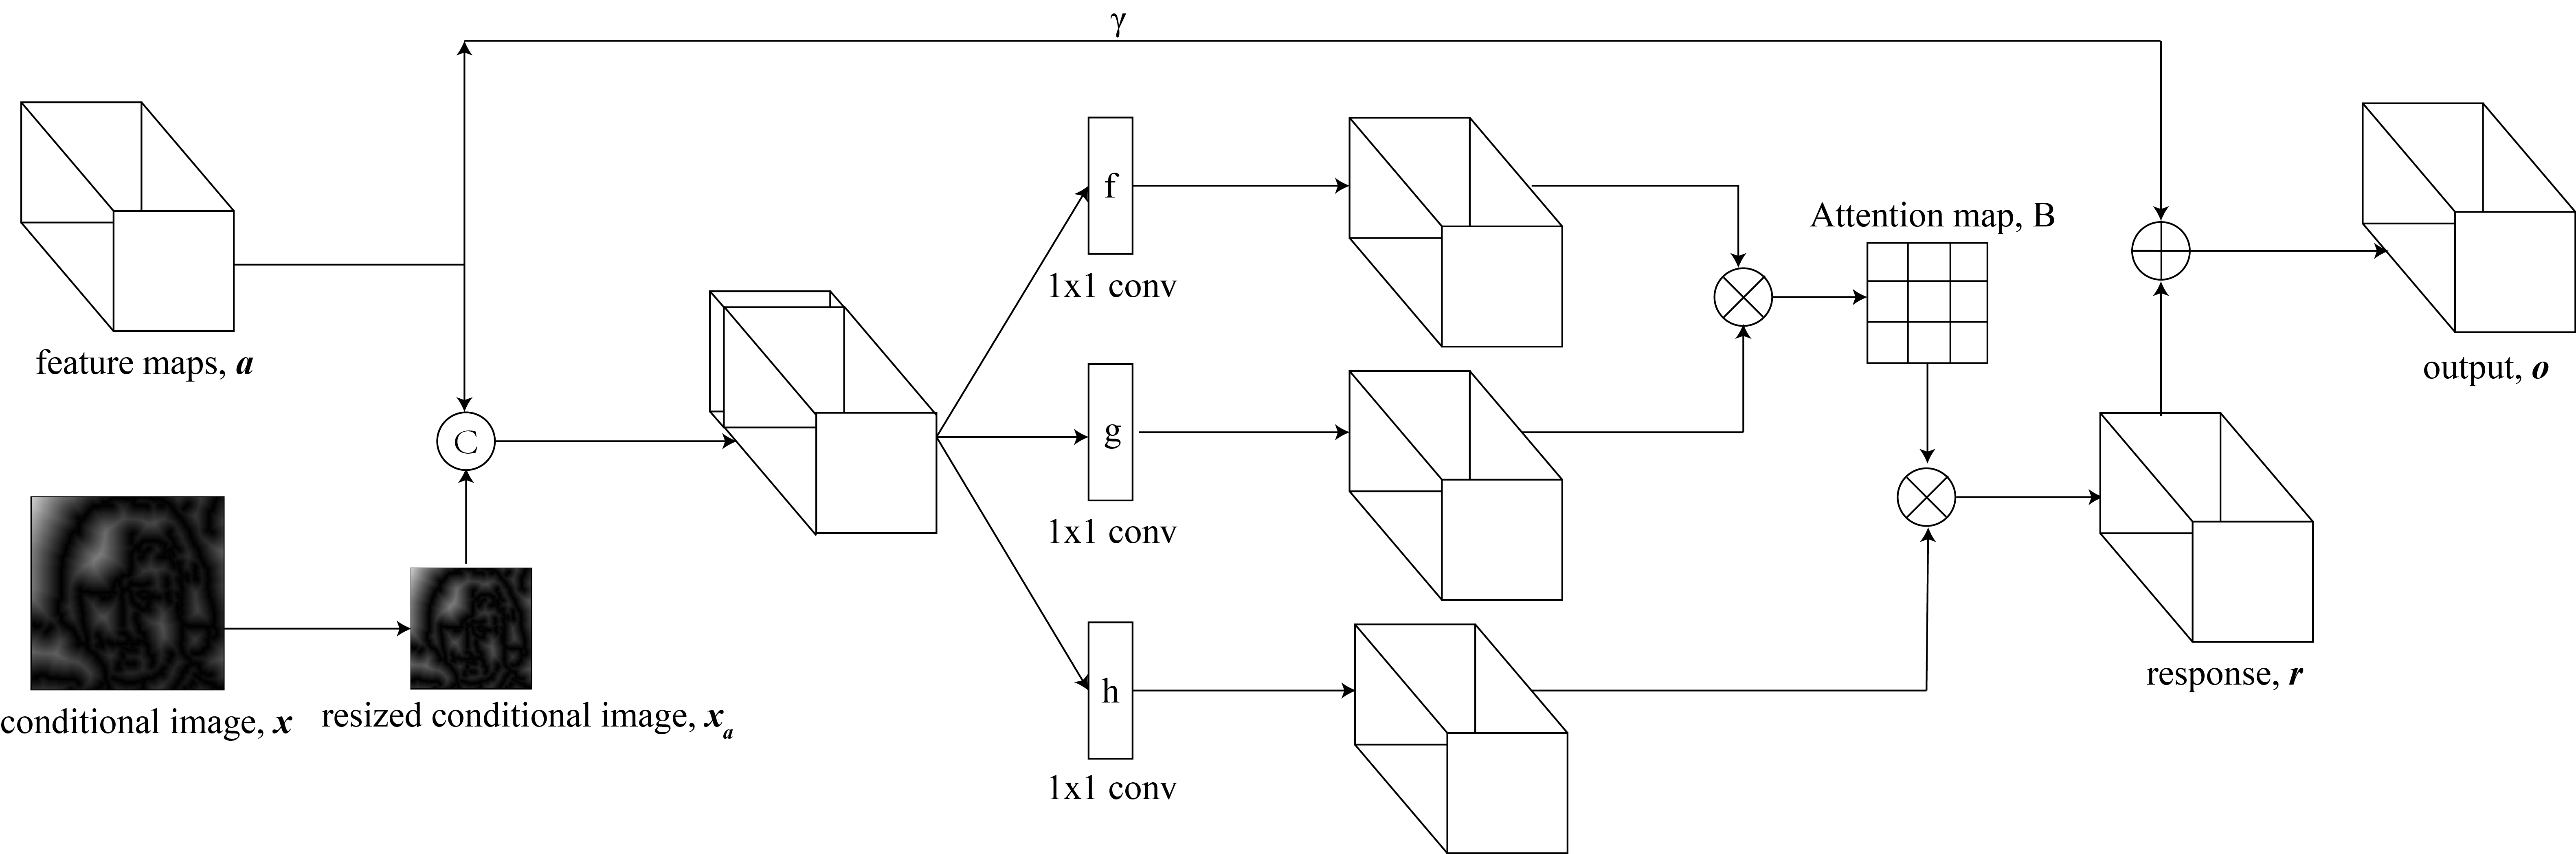
\includegraphics[width=0.8\textwidth]{figures/CSAM}
	\caption{The proposed CSAM. Given the conditional image and feature maps from the previous layer, the output feature maps are calculated in a self-attention manner. This module is designed to be added after any assigned layers.}
	\label{fig:CSAM}
\end{figure}
%
%
\subsection{Conditional Self-Attention Module (CSAM)}
\label{subsec:CSAM}
We improve the pix2pix model by utilizing self-attention mechanism to capture the long-range dependencies of images and feature maps. A recently proposed method \cite{SAGANs} has introduced self-attention to unconditional GANs and achieved state-of-the-art results. Inspired by this method, we propose a conditional self-attention module (CSAM) which is suitable for image-to-image translation framework and able to leverage the conditional information directly. This module is designed as a general module of conditional frameworks and can be added after any existing modules. We will provide details of our architecture in Subsection \ref{subsec:architecture}. The formulation of CSAM is described below.

% $\boldmath{x} \bold{x} \mathbf{x} \mathbm{x} \vec{x}$
% TODO: notation of vectors and matrices, images and feature maps 
Given the conditional image $\bm{x}\in \mathbb{R}^{3\times N_{\bm{x}}}$ and feature maps from the previous layer $\bm{a}\in \mathbb{R}^{C\times N_{\bm{a}}}$, we first resize the conditional image $\bm{x}$ to match the size of $\bm{a}$ and get $\bm{x}_{\bm{a}}\in \mathbb{R}^{3\times N_{\bm{a}}}$. Here $N_{\bm{x}}=H_{\bm{x}}\times W_{\bm{x}}$, where $H_{\bm{x}}, W_{\bm{x}}$ are the height and width of the conditional image $\bm{x}$. $N_{\bm{a}}$ is defined similarly for $\bm{a}$.
Then we concatenate the resized conditional image $\bm{x}_{\bm{a}}$ to the feature maps $\bm{a}$ to get $[\bm{a}, \bm{x}_{\bm{a}}]$ as conditioned features, where $[\cdot,\cdot]$ is the concatenation operation. This allows the information of conditional image to convey to every attention module and guide the network to form the attention directly based on the conditional image.
%

In order to calculate the attention, we map the conditional features $[\bm{a}, \bm{x}_{\bm{a}}]$ to two feature spaces by:
\begin{equation}
\label{eqn:f}
f([\bm{a}, \bm{x}_{\bm{a}} ])=\mathbf{W}_f[\bm{a}, \bm{x}_{\bm{a}} ],
\end{equation}
\begin{equation}
\label{eqn:g}
g([\bm{a}, \bm{x}_{\bm{a}} ])=\mathbf{W}_g[\bm{a}, \bm{x}_{\bm{a}} ],
\end{equation}
where $W_f, W_g\in \mathbb{R}^{\hat{C}\times (C+3)}$ are trainable weights and are implemented by $1\times 1$ convolutions. Here, we use $\hat{C}=C/8$ in our experiments following the setting of previous work \cite{SAGANs}.
%
Let $\mathbf{B}\in \mathcal{R}^{N_{\bm{a}}\times N_{\bm{a}}}$ be the attention map. Every element in $\mathbf{B}$ is denoted as $b_{j,i}$ which indicates the extent to which the model attends to the $i^{th}$ location when synthesizing the $j^{th}$ region and is calculated by 
\begin{equation}
\label{eqn:beta}
b_{j,i}=\frac{exp(s_{ij})}{\sum^{N_a}_{i=1}exp(s_{ij})}
\end{equation}
where $s_{ij}=f([\bm{a}, \bm{x}_{\bm{a}} ])^Tg([\bm{a}, \bm{x}_{\bm{a}} ])$. Next, we use $b_{j,i}$ as the attention weights and compute the response $\bm{r}=(\bm{r}_1, \bm{r}_2,\cdots, \bm{r}_{N_{\bm{a}}})\in \mathbb{R}^{C\times N_{\bm{a}}}$ at every position as a weighted sum of the features at all positions, where
\begin{equation}
\label{eqn:response}
\bm{r}_j=\sum^{N_{\bm{a}}}_{i=1}b_{j,i}h([\bm{a}, \bm{x}_{\bm{a}} ]),
\end{equation}
where $h([\bm{a}, \bm{x}_{\bm{a}}])=\mathbf{W}_h[\bm{a}, \bm{x}_{\bm{a}} ]$ and $\mathbf{W}_h\in \mathbb{R}^{(C+3)\times (C+3)}$.
As suggested in \cite{SAGANs}, we further multiply the response of the attention layer by a scale parameter $\gamma$ and add back to the input feature maps. The final output is calculated by 
\begin{equation}
\label{eqn:output}
\bm{o}_i=\gamma \bm{r}_i+\bm{a}_i,
\end{equation}
where $\gamma$ is trainable value and is set to $0$ at the beginning of the training process. This is because at the early stage of training process, the networks are able to learn the local dependencies, and then learn the long-range dependencies by assign more weight to the non-local evidence progressively.
%
%
\subsection{Multi-Level Patch Discriminator}
\label{subsec:disciminator}
The discriminator of the pix2pix model is patch-wised, which distinguishes the real/synthesized images patch by patch convolutionally with in a local receptive field much smaller than the size of the input images. 
The average value of all responses is provided as the ultimate output of $d$. 
This is based on the assumption of independence between pixels separated by more than a patch diameter. 
However, since the structural constrain is global information across the entire image, the patch-wise discriminator lacks ability to capture this global information.
We add another global discriminator $D_g$ with a receptive field as large as the entire image to capture the global structure information. The patch discriminator $D_p$ and the global discriminator $D_g$ share weights in first few layers since the lower features of these discriminators should be the same, as shown in Figure \ref{fig:architecture}. The objective of the minmax game therefore is modified from Equation \ref{eqn:minmax_game} to
\begin{equation}
\label{eqn:new_minmax_game}
\min_G \max_{D_g, D_p} \mathcal{L}_{adv}(G;D_g,D_p)+\lambda \mathcal{L}_{L1}(G),
\end{equation}
where the adversarial loss is given by 
\begin{equation}
\label{eqn:new_loss_adv}
	\begin{aligned}
	\mathcal{L}_{adv}(G;D_g,D_p)&=E_{(\bm{x},\bm{y})\sim p_{data}(\bm{x},\bm{y})}[\log D_g(\bm{x},\bm{y})+\log D_p(\bm{x},\bm{y})] \\
	&+E_{\bm{x}\sim p_{data}(\bm{x})}[\log(1-D_g(\bm{x},G(\bm{x})))+\log(1-D_p(\bm{x},G(\bm{x})))],
	\end{aligned}
\end{equation}
and $L_1$ loss is still the same as Equation \ref{eqn:loss_l1}.
%
%
\subsection{Architecture}
\label{subsec:architecture}
% add CSAMs to discriminator or not? if not, why? (GPU memory budget limited)
Our architecture, shown in Figure \ref{fig:architecture}, is based on that of the pix2pix method which uses a convolution-based U-Net \cite{Unet} as its generator and a patch-wise discriminator. We add a proposed CSAM after every convolutional layer of the generator except the first and last ones. The conditional image is resized to specific size and concatenate to the previous feature maps as the input of every CSAM. CSAMs are able to access the information of the conditional image directly and model the long-range dependencies across images and feature maps. Also, we switch the patch-wise discriminator into the proposed multiple level patch discriminator to enable the discriminator network to capture both global and local information and therefore guide the generator to generate images with more structural layout. More details of the architecture are discussed below.
%
\begin{figure}
	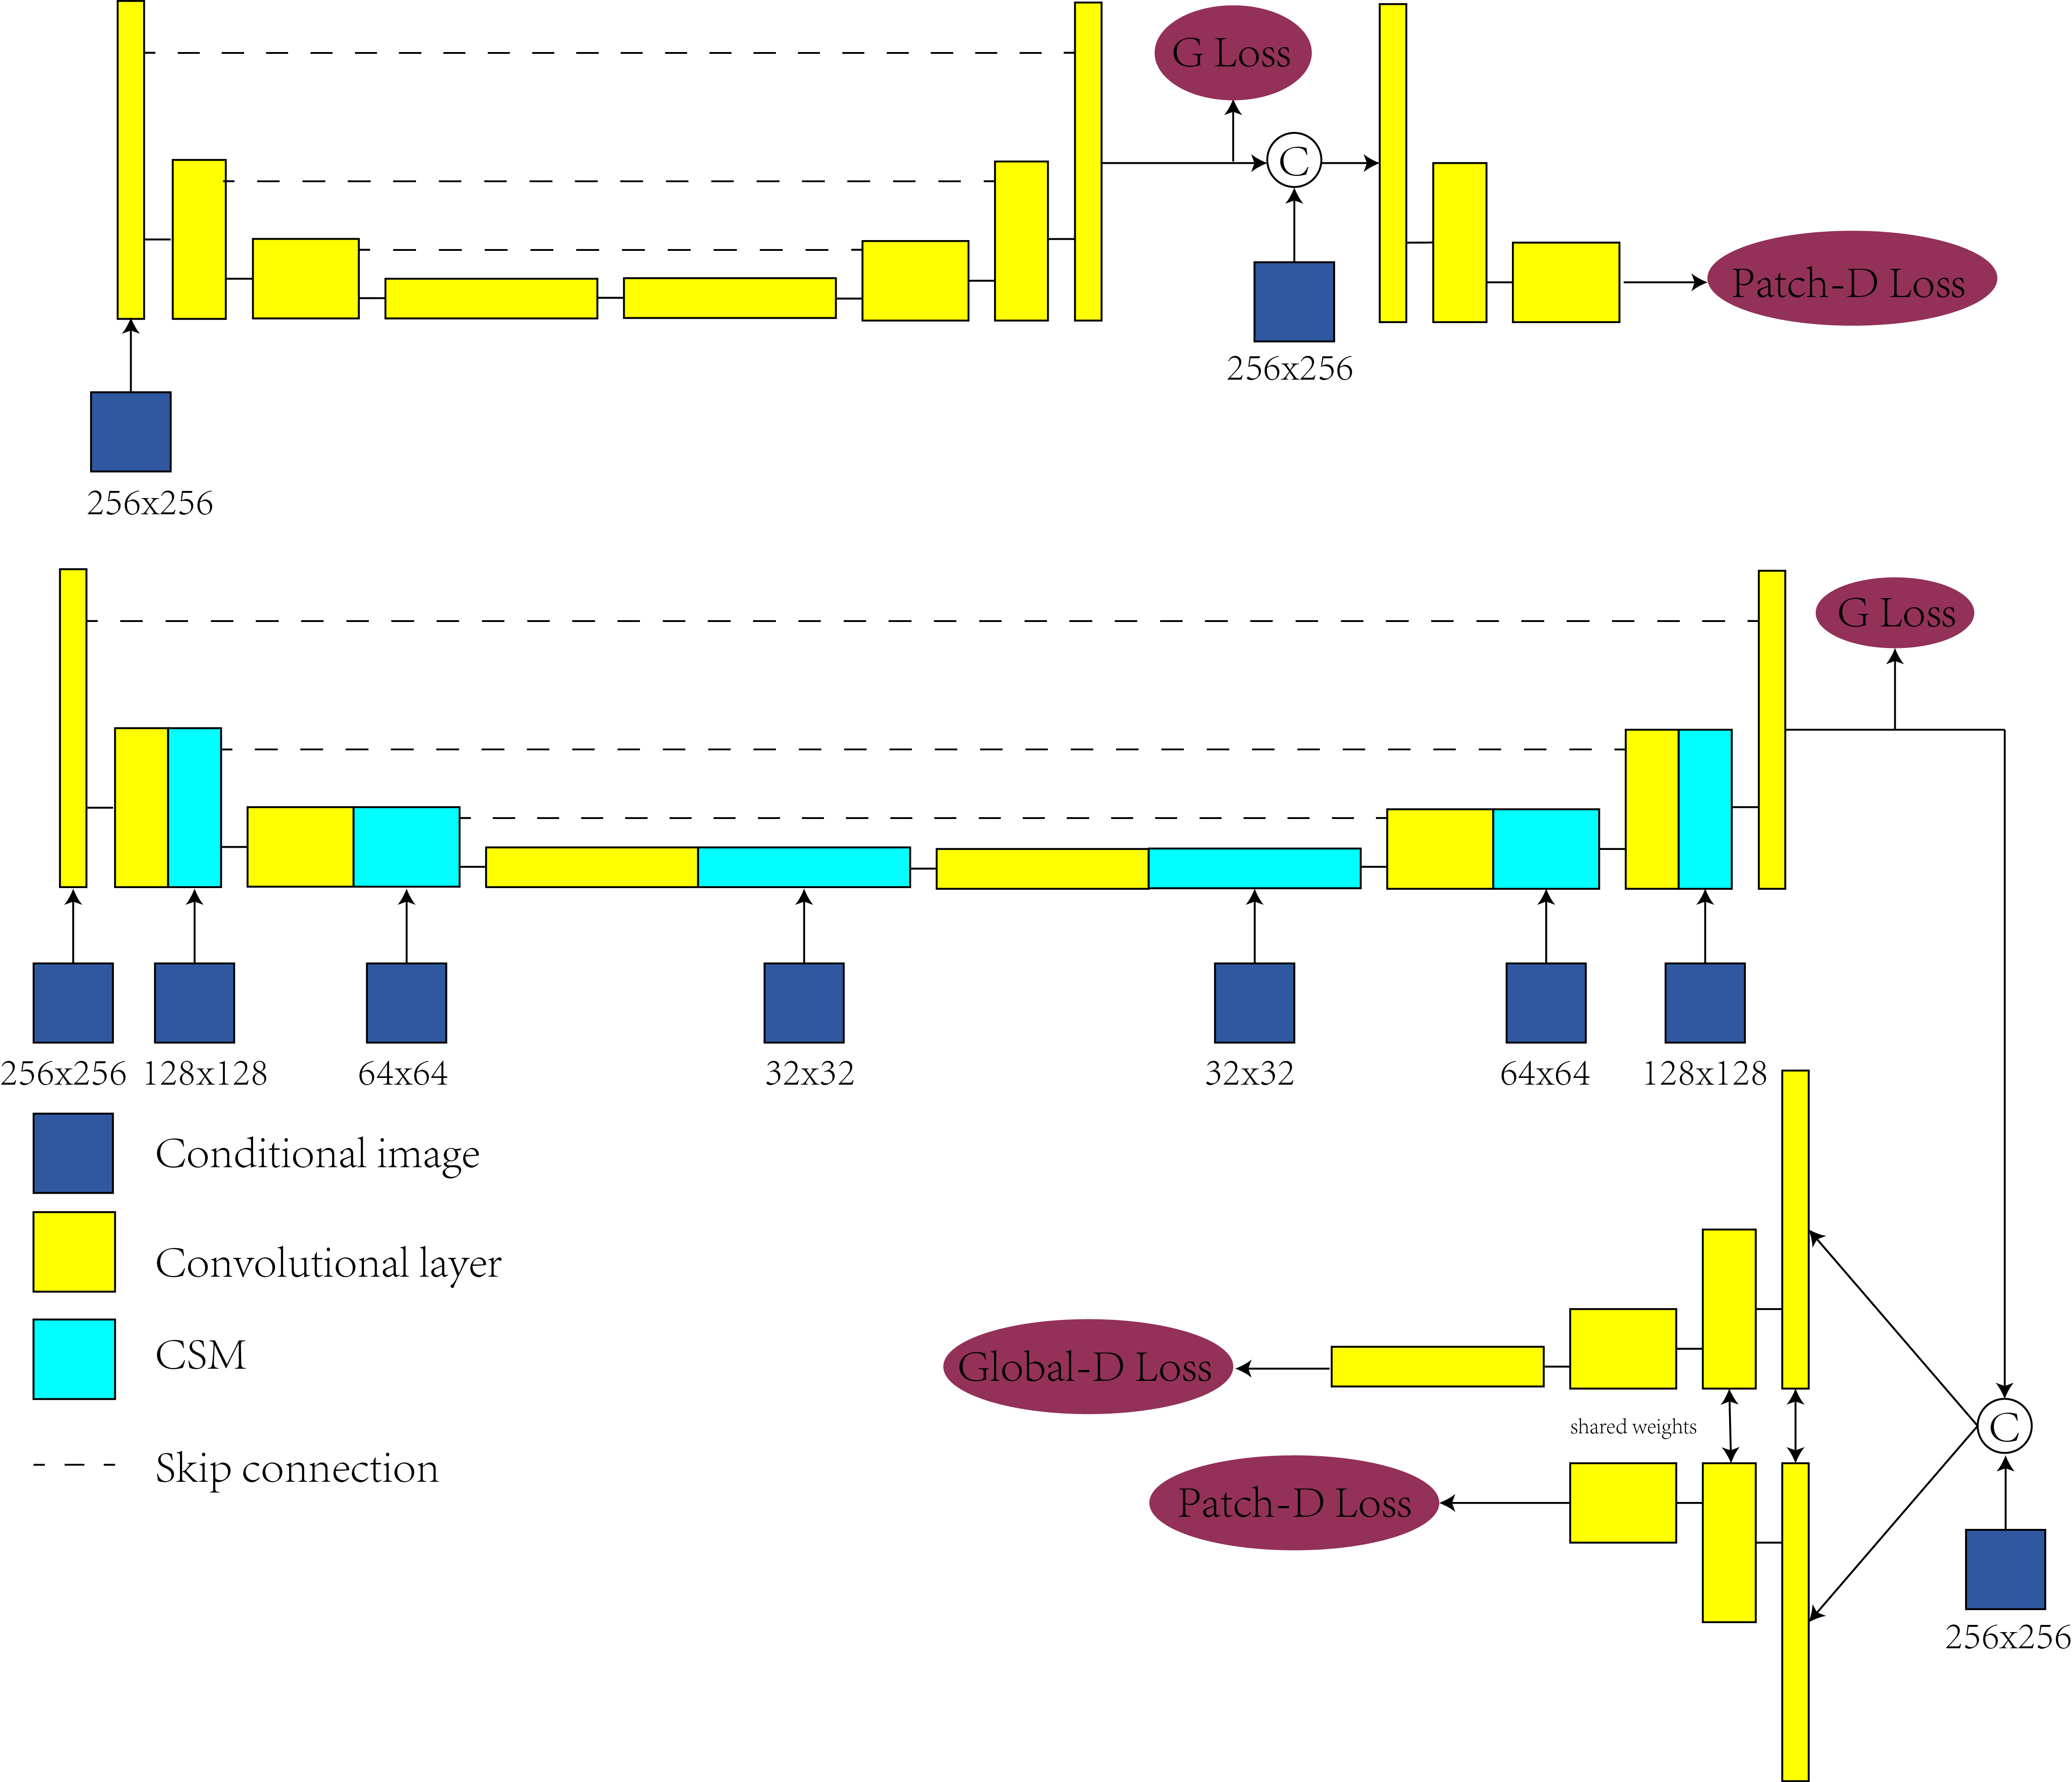
\includegraphics[width=0.8\textwidth]{figures/architecture}
	\caption{The pix2pix framework (the upper architecture) and the proposed framework (the lower architecture). Compared to the pix2pix model, in the generator of CSAGAN CSAMs are added after every convolutional layers except the first and the last ones. The discriminator is changed into a multi-level discriminator. The conditional image is resized and connect to every CSAM in the generator.}
	\label{fig:architecture}
\end{figure}
%
%
\paragraph{Noise vector} Some past conditional GANs add a noise vector to the generator as input to avoid it producing a deterministic output. However, the pix2pix model has shown that the noise vector is just ignored by the generator network and hardly change the output samples. We observe the same phenomenon in our experiments and do not apply the noise vector in our model. 
\paragraph{Spectral Normalization} Spectral normalization \cite{SN} is a recently proposed normalization technique, which restricts the spectral norm of each layer of the discriminator to constrain its Lipschitz constant. Spectral normalization is computationally efficient and require no extra hyper-parameter. It has shown that spectral normalization also benefit the training of generator by avoiding unusual gradients. We add spectral normalization to the discriminator and CSAMs in the generator.
%